\documentclass[tikz,border=5pt]{standalone}
\usepackage{tikz}
\usetikzlibrary{arrows.meta, positioning, calc, shapes.geometric, fit}

\begin{document}

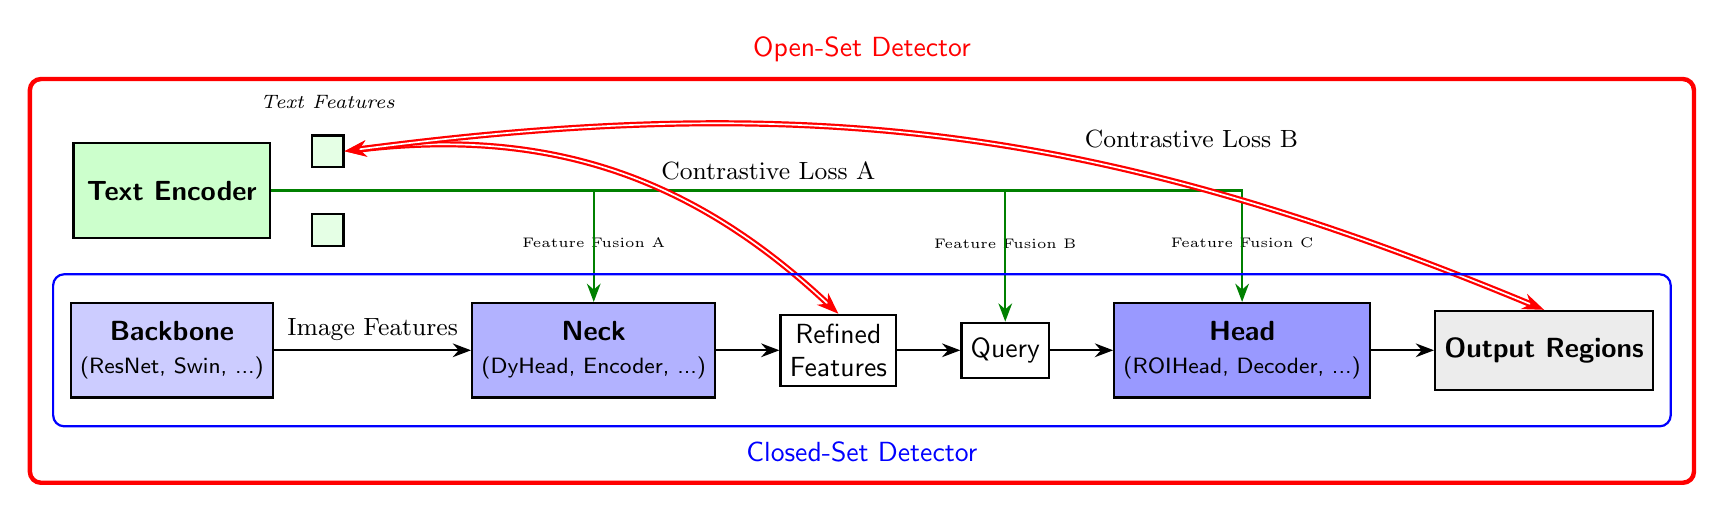
\begin{tikzpicture}[
    font=\sffamily,
    node distance=2.5cm,
    >=Stealth,
    every node/.style={align=center}
]

%-------------------------------
% 1) Main Pipeline (Horizontal)
%-------------------------------
\node[draw, thick, rectangle, fill=blue!20,
      minimum width=2.5cm, minimum height=1.2cm] (backbone)
      {\textbf{Backbone}\\\footnotesize (ResNet, Swin, ...)};
\node[draw, thick, rectangle, fill=blue!30,
      minimum width=2.5cm, minimum height=1.2cm,
      right=2.5cm of backbone] (neck)
      {\textbf{Neck}\\\footnotesize (DyHead, Encoder, ...)};




%--------------------------------
% 2) Text Encoder and Text Features (Upper Left)
%--------------------------------
\node[draw, thick, fill=green!20,
      minimum width=2.5cm, minimum height=1.2cm,
      above=0.8cm of backbone] (textenc)
      {\textbf{Text Encoder}};

% Text Features squares above the Text Encoder
\node[draw, thick, fill=green!10, rectangle,
      minimum width=0.4cm, minimum height=0.4cm,
      right=0.5cm of textenc.east, yshift=-0.5cm] (txtA) {};
\node[draw, thick, fill=green!10, rectangle,
      minimum width=0.4cm, minimum height=0.4cm,
      right=0.5cm of textenc.east, yshift=0.5cm] (txtB) {};
\node[above=0.2cm of txtB, font=\scriptsize\itshape] {Text Features};

%-----------------------------------
% 3) Feature Fusion Boxes A, B, C
%-----------------------------------
\node[draw, thick, rectangle, fill=white,
      minimum width=0.7cm, minimum height=0.7cm,
      right=0.8cm of neck] (fusA) {Refined\\ Features};
\node[above=16pt of neck.north, font=\tiny] {Feature Fusion A};

\node[draw, thick, rectangle, fill=white,
      minimum width=0.7cm, minimum height=0.7cm,
      right=0.8cm of fusA] (fusB) {{Query}};
\node[above=23pt of fusB, font=\tiny] {Feature Fusion B};

\node[draw, thick, rectangle, fill=blue!40,
      minimum width=2.5cm, minimum height=1.2cm,
      right=0.8cm of fusB] (head)
      {\textbf{Head}\\\footnotesize (ROIHead, Decoder, ...)};


\node[above=16pt of head, font=\tiny] {Feature Fusion C};

\node[draw, thick, rectangle, fill=gray!15,
      minimum width=2.4cm, minimum height=1.0cm,
      right=0.8cm of head] (output)
      {\textbf{Output Regions}};

%-------------------------------------------
% 4) Connections from Text Encoder to Fusion Boxes
%-------------------------------------------
% Arrow to A: Downward and then right
\draw[->, thick, green!50!black] (textenc.east) -- ++(0.2, 0 cm) -| (neck.north);

% Arrows to B and C: Bending left from east edge
\draw[->, thick, green!50!black] (textenc.east) -- ++(0.2, 0 cm) -|  (fusB.north);
\draw[->, thick, green!50!black] (textenc.east) -- ++(0.2, 0 cm) -|  (head.north);

% Arrows in the pipeline
\draw[->, thick] (backbone.east) -- node[above, midway, font=\small] {Image Features} (neck.west);
\draw[->, thick] (fusA.east) -- node[above, midway, font=\small] { } (fusB.west);
\draw[->, thick] (head.east) -- (output.west);

%------------------------------------------
% 5) Connections from Pipeline to Fusion Boxes
%------------------------------------------
\draw[->, thick] (neck.east) -- (fusA.west);
\draw[->, thick] (fusB.east) -- (head.west);

%--------------------------------------
% 6) Contrastive Loss Arrows (Red)
%--------------------------------------
\draw[red, thick, -Stealth, bend right=25, double, <->] (fusA.north) to
    node[midway, right, black, font=\small, xshift=0.5cm] {Contrastive Loss A} (txtB.east);
\draw[red, thick, -Stealth, bend right=15, double, <->] (output.north) to
    node[midway, right, black, font=\small, xshift=1.5cm] {Contrastive Loss B} (txtB.east);

%----------------------------------------------------
% 7) Bounding Boxes for Closed-Set / Open-Set Detectors
%----------------------------------------------------
% Closed-Set Detector: Encloses Backbone, Neck, Head, Output
\node[draw=blue, thick, rounded corners, inner xsep=6pt, inner ysep=10pt,
      fit=(backbone)(neck)(head)(output),
      label={[blue, below=2pt]below:Closed-Set Detector}] (closedSet) {};

% Open-Set Detector: Encloses entire diagram
\node[draw=red, ultra thick, rounded corners, inner xsep=8pt, inner ysep=20pt,
      fit=(closedSet)(textenc)(fusA)(fusB)(txtA)(txtB),
      label={[red, above=2pt]above:Open-Set Detector}] (openSet) {};

\end{tikzpicture}

\end{document}